\documentclass[a4paper,12pt]{article}
\usepackage[indonesian]{babel}
\usepackage{graphicx}
\usepackage{multirow}
\usepackage{enumitem}
\usepackage{listings}
\usepackage{wrapfig}
\usepackage[T1]{fontenc}
\usepackage{inconsolata}
\usepackage{lipsum}
\usepackage{adjustbox}


\usepackage{color}
\usepackage[table]{xcolor}
\definecolor{mygreen}{rgb}{0,0.6,0}
\definecolor{mygray}{rgb}{0.5,0.5,0.5}
\definecolor{mymauve}{rgb}{0.58,0,0.82}
\lstset{%
    language=java,
    showstringspaces=false,          % Prevent tex replacing space to bracket in code
    frame=single,                    % Set frame around code
    backgroundcolor=\color{white},   % choose the background color
    basicstyle=\footnotesize,        % size of fonts used for the code
    breaklines=true,                 % automatic line breaking only at whitespace
    captionpos=b,                    % sets the caption-position to bottom
    commentstyle=\color{mygreen},    % comment style
    keywordstyle=\color{blue},       % keyword style
    stringstyle=\color{mymauve},     % string literal style
    numbers=left,
}

\graphicspath{ {./img/} }
\begin{document}
\title{ {\Large Laporan Praktikum}\\ Analisis dan Desain Sistem\\{\Large Pertemuan 1}}

\author{Aldzikri Dwijayanto Prathama
    \\195410189
    \\Informatika}
\makeatletter
\begin{titlepage}
    \begin{center}
        {\huge \bfseries \@title}\\[14ex]
        
\includegraphics[scale=.8]{logo}\\[4ex]
        {\large \@author}\\[12ex]
        {\large \bfseries {SEKOLAH TINGGI MANAJEMEN INFORMATIKA DAN KOMPUTER
            AKAKOM YOGYAKARTA}}
    \end{center}


%{\large \@date}
\end{titlepage}
\makeatother
%\maketitle
\newpage
\tableofcontents
\newpage

\section{Tujuan}
Mahasiswa mampu menjelaskan sebuah sistem sesuai klasifikasi system dan mampu menyebutkan komponen-komponen sebuah
sistem
\section{Teori}
Sistem adalah sekumpulan elemen yang saling terkait atau terpadu untuk mencapai tujuan tertentu.Penjelasan untuk
masing-masing elemen
\begin{enumerate}
    \item Tujuan: segala sesuatu yang akan diraih atau dituju oleh sebuah sistem 
    \item Masukan: Segala sesuatu yang masuk ke dalam sistem. Sesuatu yang masuk ke dalam sistem bisa
        berwujud (bahan mentah) maupun tidak berwujud (data/informasi)
    \item Proses: mentransformasikan masukan menjadi keluaran
    \item Output: hasil pemrosesan (bisa berupa: informasi, saran, laporan, produk tertentu)
    \item Mekanisme pengendalian dan umpan balik: mengendalikan masukan dan proses sehingga sistem dapat berjalan sesuai tujuan
    \item Batasan (boundary): pemisah antara sistem dengan luar sistem (lingkungan) atau membatasi sub
        sistem dengan sub sistem yang lain
    \item Lingkungan (environment): segala sesuatu yang berada di luar sistem yang mempengaruhi kerja sistem 
\end{enumerate}

Sistem dapat diklasifikan sebagai berikut:
\begin{enumerate}
   \item sistem abstrak dan sistem fisik
   \item sistem deterministik dan sistem probabilistic
   \item sistem tertutup dan sistem terbuka
   \item sistem alami dansistem buatan manusia
   \item sistem sederhana dan sistem kompleks 
\end{enumerate}

Sistem abstrak: sistem yang berisi gagasan atau konsep tertentu. contoh: sistem teologi (hubungan manusia dan tuhan),
ideologi tertentu. Sedangkan sistem fisik: tampak secara fisik.\\
Sistem    deterministicadalah  sistem  dimana  operasi    dan    hasilnya    dapat    diprediksi  secara    tepat,
sedangkan sistem probabilistic adalah sebuah sistem yang tidak dapat diprediksi secara tepat karena mengandung
unsur probabilistik (contoh: sistem persediaan barang, arisan)\\
Sistem tertutup(relatif tertutup):sistem yang tidak menerima Pengaruh dari lingkungan luar memiliki
masukan dan keluaran tertentu. Sistem terbuka: sistem yang dapat menerima pengaruh dari lingkungan  
luar dan dapat beradaptasi tehadap lingkungan.\\
Sistem alami adalah sebuah sistem yang sudah ada secara alamiah, sedangkan system buatan manusia adalah sistem yang
sengaja dibuat oleh manusia.
\newpage

\section{Pembahasan}
\subsection{Praktik}
Pada praktik mahasiswa mempelajari sistem STMIK AKAKOM, mulai dari klasifikasi dan elemen dari sistem STMIK AKAKOM.
Dilihat dari elemen Masukan yaitu calon mahasiswa ini merupakan sesuatu yang berwujud dan memiliki nilai data maupun informasi. Kemudian pada elemen Proses yaitu perkuliahan yang ditempuh mahasiswa. Keluaran yaitu menghasilkan Lulusan.
\begin{center}
    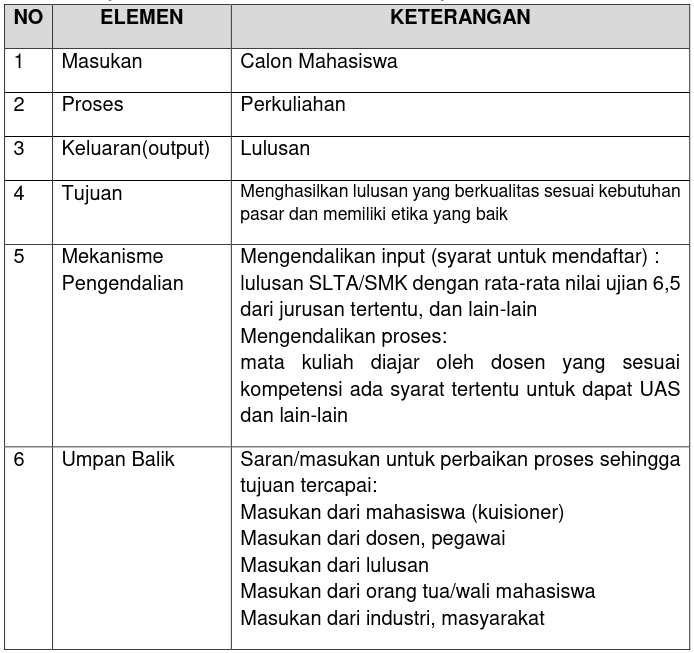
\includegraphics[width=\textwidth]{tbl1} 
\end{center}
\begin{itemize}
    \item Boundary System (batasan system): perguruan tinggi yang lain
    \item Lingkungan (environment): pemerintah, pihak industry, masyarakat
\end{itemize}
Penjelasan berdasarkan klasifikasi system:\\
\begin{itemize}
   \item STMIK AKAKOM dapat diklasifikan sebagai sistem fisik, karena memiliki bangunan, dosen, mahasiswa, dll yang
       wujudnya nyata
    \item STMIK AKAKOM dapat diklasifikan sebagai sistem terbuka karena menerima masukan dari luar, seperti regulasi
        pemerintah, masukkan mahasiswa, atau alumni.
    \item STMIK AKAKOM dapat diklasifikan sebagai sistem buatan manusia, karena sengaja didirikan oleh manusia.
\end{itemize}

\begin{center}
    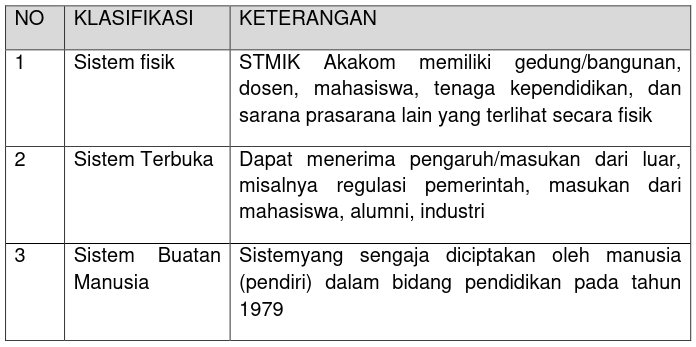
\includegraphics[width=\textwidth]{tbl2}
\end{center}

\newpage
\subsection{Latihan}
\begin{enumerate}
   \item Pada latihan ini Berikan penjelasan mengapa STMIK Akakom dapat diklasifikasikan sebagai sistem yang
       deterministik?\\
        Ya karen STMIK Akakom sudah membentuk kesatuan antara satu komponen dengan satu komponen lainnya menjadi suatu
        sistem, yang komponen dari sistem tersebut beroperasi dengan hasil yang dapat diperkirakan
        secara tepat, yang masing-masing komponennya berinteraksi untuk menghasilkan keluaran. Tujuan dari sistem
        tersebut memiliki akhir tujuan yang tepat untuk setiap perkara atau kasus yang terjadi dalam setiap sistem
        tersebut. Sehingga STMIK Akakom dapat diklasifikasikan menjadi Sistem Deterministik.
    \item Dalam Elemen sistem ‘STMIK Akakom’, apakah dosen dapat dimasukkan ke dalam elemen sistem? Beri penjelasan!\\
        Ya karena dosen merupakan bagian dari sistem STMIK AKAKOM, yang tepatnya sistem fisik karena berwujud nyata, dan
        memiliki peran dalam menghasilkan keluaran.
\end{enumerate}

\subsection{Tugas}

\section{Kesimpulan}
\end{document}
